\documentclass[a4paper]{report}
\usepackage[T1]{fontenc} % Fontes T1
\usepackage[utf8]{inputenc} % Input UTF8
\usepackage[backend=biber, style=ieee]{biblatex} % para usar bibliografia
\usepackage{csquotes}
\usepackage[portuguese]{babel} %Usar língua portuguesa
\usepackage{blindtext} % Gerar texto automaticamente
\usepackage[printonlyused]{acronym}
\usepackage{hyperref} % para autoref
\usepackage{graphicx}
\usepackage{float}
\usepackage{indentfirst}

\bibliography{bibliografia}


\begin{document}
%%
% Definições
%
\def\titulo{As Causas Do Comportamento Humano Na Inteligência Artificial Dentro De Vídeo Jogos}
\def\data{25 de dezembro de 2023}
\def\autores{Matheus Pinto, Henrique Moreira}
\def\autorescontactos{(118621) matheusp@ua.pt, (119809) henriquemm04@ua.pt}
\def\codeualink{https://github.com/detiuaveiro/infor2023-ap-g-infor2023-ap-g41}
\def\versao{V1.0}
\def\departamento{DETI - Universidade de Aveiro}
\def\empresa{Universidade de Aveiro}
\def\logotipo{ua.pdf}
%
%%%%%% CAPA %%%%%%
%
\begin{titlepage}

\begin{center}
%
\vspace*{50mm}
%
{\Huge \titulo}\\ 
%
\vspace{10mm}
%
{\Large \empresa}\\
%
\vspace{10mm}
%
{\LARGE \autores}\\ 
%
\vspace{30mm}
%
\begin{figure}[h]
\center
\includegraphics{\logotipo}
\end{figure}
%
\vspace{30mm}
\end{center}
%
\begin{flushright}
\versao
\end{flushright}
\end{titlepage}

%%  Página de Título %%
\title{%
{\Huge\textbf{\titulo}}\\
{\Large \departamento\\ \empresa}
}
%
\author{\autores\\\autorescontactos\\
    \\
GIT: \codeualink}
%
\date{\data}
%
\maketitle

\pagenumbering{roman}

%%%%%% RESUMO %%%%%%
\begin{abstract}
Neste trabalho, exploramos a relação entre a \ac{IA} e os videojogos, e como os humanos reagem à \ac{IA} em ambientes de jogo. Começamos por nos questionar se a IA pode ter um comportamento humano. Embora a \ac{IA} tenha avançado muito, igualar a complexidade do comportamento humano ainda é um desafio, uma vez que os humanos frequentemente agem de maneira irracional e criativa, o que as IA lógicas acham difícil.\\
    
Em seguida, concentramo-nos em saber se a \ac{IA} pode ter um comportamento humano em videojogos. Os videojogos revolucionaram a indústria do entretenimento e dependem da \ac{IA} para criar experiências desafiantes e satisfatórias. No entanto, a \ac{IA} em videojogos ainda enfrenta limitações em termos de adaptação a situações imprevistas.\\
    
Por fim, exploramos como os humanos reagem à dificuldade da \ac{IA} em videojogos. Os jogos utilizam estratégias como a dificuldade dinâmica adaptativa para equilibrar o desafio e a satisfação do jogador. Alguns jogos, como os Soulslike, tornaram-se famosos por sua alta dificuldade e geraram reações diversas nos jogadores, desde a satisfação de superar um desafio extremo até a frustração.\\
    
Em resumo, a relação entre a \ac{IA} e os videojogos é fascinante e desafiadora. À medida que a tecnologia avança, é provável que vejamos melhorias na capacidade da \ac{IA} de se adaptar aos jogadores. No entanto, a lacuna entre a \ac{IA} e o comportamento humano ainda é considerável, tornando a interação entre humanos e máquinas no mundo dos videojogos intrigante e em constante evolução.
\end{abstract}
%
\tableofcontents
%
\clearpage
\pagenumbering{arabic}
%
% Introdução
\chapter{Introdução}
\label{chap.introducao}

O comportamento humano é um conjunto de mecanismos que o ser humano utiliza para agir diante de uma série de estímulos externos, denominados (o ecossistema, a cultura e a genética), são fatores que afetam o comportamento humano para permitir que o homem se comporte de determinada maneira. racional e à sua vontade, dentro deste termo entram os debates filosóficos que tentam decifrar se o comportamento humano só existe no homem, ou também outros seres ou indivíduos poderiam optar por esse comportamento.Na Grécia antiga, filósofos como Platão e Sócrates garantiram que o humano se comportava dependendo de seu ecossistema, semelhante a um animal desenvolvido, com maior inteligência que o resto dos seres vivos da época, tudo isso foi pensado durante 20 séculos até que em 1956 John McCarthy, Marvin Minsky e Claude Shannon. Eles cunharam o termo inteligência artificial pela primeira vez na Conferência de Dartmouth.\\

Eles definiram \ac{IA} como as novas máquinas inteligentes, mais tarde isso foi alterado para o conceito mais preciso dado por Andreas Kaplan e Michael Haenlein onde ditam que é a capacidade de um sistema receber uma série de instruções para realizar uma atividade no mesmo maneira mais fácil e rápida possível. Graças a este conceito, muitas pessoas começaram a compará-lo com o comportamento dos humanos, sabendo que os seres humanos se comportam em função dos estímulos que recebem externamente, e da mesma forma que a \ac{IA} recebe estímulos e se comporta de forma a tentar cumprir um objetivo. que seu programador projetou para você.\\

As limitações deste trabalho dão-se pelo pouco material a respeito do tema devido ao fato de ser algo bastante novo e que sua verdadeira contribuição para a humanidade ainda está em dúvida, a forma de coletar informações foi lendo bastante alguns documentos da Internet, brochuras, livros, videogames e vídeos do YouTube . Este trabalho será explicativo e analítico com desenho documental.\\

A motivação do autor para realizar esta pesquisa foi explicar às pessoas como funciona a \ac{IA} e saber se elas podem se comportar como seres humanos. Levando em consideração que estes são desenhados a partir de redes neurais já sistematizadas e que em tese não deveriam mudar seu comportamento, e caso o mudem, explique suas causas em diversos contextos como, por exemplo: dentro de um videogame.\\

O trabalho busca coletar informações teóricas sobre as causas que podem fazer com que a \ac{IA} tenha comportamento humano dentro dos videogames. Respondendo a 3 perguntas divididas em capítulos: uma \ac{IA} pode ter comportamento humano? A \ac{IA} pode ter comportamento humano dentro de um sistema previamente desenvolvido, como um videogame ? e como os humanos se comportariam dependendo da dificuldade da \ac{IA} em um videogame?\\

Antes de abordar tudo relacionado ao problema, o autor quer definir os termos mais complicados de entender, seriam eles:\\

\textbf{JOGO:}
Um jogo é um tipo de atividade de entretenimento, em que os participantes tentam atingir pelo menos um objetivo arbitrário e não trivial, agindo de acordo com as regras.\\

\textbf{VÍDEO JOGO:} Videogame é uma aplicação interativa voltada para o entretenimento que, por meio de determinados comandos ou controles sistemáticos, atinge um final pré-determinado já predisposto por seus programadores.\\

\textbf{\ac{IA}:} Andreas Kaplan e Michael Haenlein dizem que “é a capacidade de um sistema interpretar corretamente dados externos, aprender com esses dados e usar esse conhecimento para alcançar tarefas e objetivos específicos através de adaptação flexível”.\\

\textbf{ALGORITMO:} sequência de instruções dadas ao resolver um problema\\

\textbf{REDE NEURONAL:} são uma série de algoritmos de aprendizagem estatística inspirados no cérebro humano. Eles são comumente usados para estimar ou aproximar funções que geralmente são desconhecidas.\\

\textbf{NPC:} mais conhecido como (NON PLAYLABLE CHARACTER), são aqueles personagens que a pessoa que está jogando um videogame não pode ocupar, na maioria das vezes estes vêm com uma programação bastante simples e ultimamente eles are emprega uma \ac{IA}, dependendo da atividade designada para ela.\\

\textbf{APRENDIZAGEM DE MÁQUINA:} este é um grupo de algoritmos que dá a uma máquina a capacidade de identificar padrões massivos para aprender ou fazer previsões, todos esses algoritmos mostram à máquina o que ela tem que fazer, este sistema foi a salvação para os programadores, pois reduziu sua carga de trabalho ao injetar informações em uma \ac{IA}.\\

\textbf{BOTÕES:} é uma instância de \ac{IA} que controla uma ou mais unidades que compartilham o mesmo cérebro virtual. Cada bot em um jogo pode ter propriedades e personalidades diferentes. Quanto aos jogadores, eles têm seus próprios objetivos, na maioria das vezes separados uns dos outros.

%%%%%%
% Realidade Virtual
\chapter{Uma \ac{IA} pode  ter comportamento humano?}\cite{ia}
%%%%%%%%
Desde que Andreas Kaplan e Michael Haenlein deram o conceito do que era a \ac{IA}, muitas pessoas começaram a perguntar-se: existe a possibilidade de se comportarem como humanos?Será que a \ac{IA} pode superar a nossa capacidade cognitiva? Essas e muitas outras perguntas têm sido feitas por pessoas ao longo dos anos, porém, ainda estamos muito longe de ter uma resposta 100\% precisa para essas incógnitas, por vários motivos, porque fazer com que uma \ac{IA} iguale ou supere as habilidades cognitivas de um ser humano ser não parece se tornar uma realidade nos próximos anos, graças à pandemia pudemos perceber  o quão importante foi o processo de digitalização para o ser humano, em todas as áreas (educacional , administrativo  , social, etc.) onde sem isso nossas vidas dentro da pandemia poderiam ter sido muito mais difíceis , para destacar isso o  autor quer dizer que muitas das atividades realizadas pela digitalização são realizadas por algoritmos , por exemplo : quando se entra sempre no Instagram aparece uma série de fotos , essas fotos aparecem dependendo se o algoritmo as determina como virais ou, na falta disso, que você pode gostar, e o algoritmo sabe disso graças ao aprendizado de máquina .\\
    
Muitos acreditam que graças ao aprendizado de máquina , o futuro da \ac{IA} seria recriar futuros apocalípticos tão bem feitos em filmes, quadrinhos e livros. o que hoje é muito pouco viável (embora existam alguns exemplos não tão drásticos em que a \ac{IA} às vezes tende a ser mais autônoma do que deveria), na realidade o verdadeiro futuro que se espera para a \ac{IA} é que eles alcancem inteligência semelhante à nossa onde no opinião do autor que seria quase como se tornar um deus, pois o que mais seria diferente de criar vida. O autor também gostaria de apresentar os possíveis estágios que podem ocorrer para as \ac{IA} no futuro.\\
    
ESTÁGIOS DA \ac{IA} NO FUTURO  :
\begin{itemize}
\item \textbf{A)} A primeira seria a etapa especializada de \ac{IA}, onde um modelo de \ac{IA} é capaz de resolver um problema muito complexo com muita eficiência, algo que vem sendo trabalhado há muitos anos.
\item \textbf{B)} Em segundo lugar, a fase de \ac{IA} cognitiva permite que modelos e máquinas tenham capacidades cognitivas próximas das dos humanos, como já foi visto com alguns robôs que até venceram concorrentes humanos em programas de televisão.
\item \textbf{C)} A terceira fase seria chamada de \ac{IA} ampla, na qual diferentes modelos são misturados para encontrar soluções complexas para problemas mais amplos. Aqui, um exemplo seria o carro autônomo.
\item \textbf{D)} Em quarto lugar ficaria a etapa da \ac{IA} associada à biotecnologia e à cibertecnologia , com modelos de habilidades cognitivas para aumentar ou melhorar as capacidades humanas, como poderia ocorrer no campo da neurocirurgia, onde um robô com conexão remota pode ajudar e fornecer precisão, entre outras, outras virtudes, às operações.
\item \textbf{E)} E, finalmente, a fase geral da \ac{IA}, onde as capacidades humanas seriam igualadas ou mesmo superadas. Isso, segundo especialistas, poderá acontecer dentro de 50 anos, no mínimo.
\end{itemize}

Respondendo à pergunta  de forma mais precisa, já tendo investigado muito sobre o que a \ac{IA} pode se tornar no futuro, sendo bastante radical, o autor deve assegurar que é muito difícil para a \ac{IA} ter comportamento humano, mais do que tudo pelo fato . que os humanos chegam a um ponto em que se tornam bastante irracionais, e ações muito fáceis como gritar ou ser insular são feitas de uma forma totalmente irracional e ilógica, o que para um robô superinteligente com \ac{IA} superdesenvolvida em 2070 seria algo quase impossível , até porque o que se pede à \ac{IA} é que seja muito lógica e realize as atividades da forma mais fácil e rápida possível.
Do ponto de vista científico nunca se pode refutar completamente algo, porque é para isso que serve a ciência, para estudar coisas que podem ou não ser uma realidade quando demonstradas e utilizadas no dia a dia.\\
    
Para deixar claro porque hoje a \ac{IA} não pode ter o comportamento humano dentro de um contexto mais geral, o pesquisador quer dar um exemplo prático:
Uma série de indivíduos querem fazer uma música , quem faz é o compositor, a maioria dos compositores tendem a ser pessoas com muita criatividade e talento, o problema é que sendo muito criativo você perde um pouco da noção da música. lógica, pois está cientificamente comprovado que as pessoas mais criativas não são tão racionais ou lógicas na hora de criar algo, neste caso a música , para uma \ac{IA} criar uma música ao nível do compositor (já tendo programado todos os parâmetros fazer uma música) seria praticamente impossível hoje, porque a \ac{IA} é muito lógica e neste caso a música  seria muito monótona ou muito vazia se comparada à do compositor muito criativo.
Neste exemplo poderíamos ver as diferenças entre um ser humano e uma máquina inteligente , o fato de que os humanos podem ser um pouco mais irracionais à vontade onde a \ac{IA} não pode , mesmo uma máquina com aprendizado de máquina não poderia ser tão criativa quanto um ser humano , agora estamos em 2021, não se sabe se até o ano 2100 será criado um novo sistema que permita que as máquinas não sejam tão racionais na hora de realizar uma atividade, por isso na ciência nunca se pode refutar nada.




%%%%%%%%
\chapter{A \ac{IA} pode ter comportamento humano dentro de um sistema previamente desenvolvido, como um videogame?}\cite{ia1}

Depois de aprender que a \ac{IA} por si só é muito difícil  de alcançar o comportamento humano, a mesma pergunta está agora a ser colocada num contexto mais específico, como os videojogos. Esta indústria cresceu muito dentro da cultura popular nas últimas décadas e revolucionou usuários de todas as idades , tendo grandes influências positivas em seus consumidores e principalmente na economia mundial, deixando de lado mercados tão fortes como o cinema ou a televisão, pois as opções de realidade aumentada ( como os óculos de realidade virtual e a constante evolução gráfica e narrativa ) colocaram esta indústria no topo do sector do entretenimento audiovisual, há um gráfico feito pela Statista Digital Market Outlook onde explicam quais são as principais ingresos do mercado de videogames.\\ 

\begin{figure}
    \center
    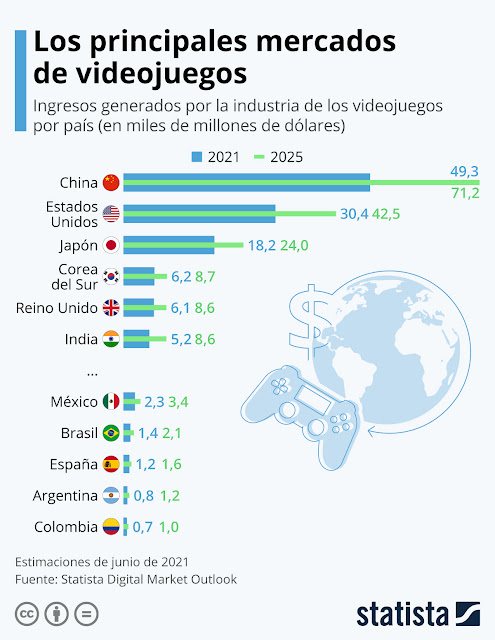
\includegraphics[width=350pt]{imagens/tabela.jpg}
    \caption{principais mercados nos videogames}~\cite{statista}
    \label{fig:chainimage}
\end{figure}

    
O dado importante é que a China e os Estados Unidos são os que  mais consomem videogames, com renda total ou superior a 27 bilhões de dólares para os asiáticos, e mais de 25 bilhões de dólares para os americanos, além de jogos mobile para smartphones ou tablets são os que dominam o mercado, com 42\% do total (mais de 46 mil milhões de dólares) seguidos das consolas, com 31\% das receitas do mercado superiores a 33 mil milhões de dólares.
A indústria dos videojogos  teve no segundo maior mercado (os Estados Unidos) em 2016 foi de mais de 11 mil milhões de dólares no produto interno bruto do país. Nos Estados Unidos, existem pouco mais de 65 mil trabalhadores empregados diretamente por desenvolvedores e produtoras de videogames, com salário médio superior a 90 mil dólares anuais.\\\\
    
Do lado latino-americano, a maior receita da indústria de videogames está no México, com mais de 1,4 bilhão de dólares e posicionando-se na 12ª posição global, seguido pelo Brasil na posição 13, Argentina na 25ª e Peru na 51ª. lugar, este último com receitas superiores a 138 milhões de dólares.
E isso só em 2016, imagine isso na pandemia onde o percentual aumentou consideravelmente por conta de ficar em casa.
Antes de poder investigar a resposta ao mistério, o autor quer explicar como funciona a \ac{IA} nos videogames.\\
    
A IA é implementada em videogames graças a algoritmos projetados com aprendizado de máquina , esses algoritmos aprendem a tomar decisões estratégicas em cenários variáveis e complicados automaticamente. Testar esses algoritmos em ambientes simulados permite que os programadores aprendam com os erros. Da mesma forma, permitem-lhes reforçar as estratégias necessárias à sua eficácia. Para conseguir isso, as simulações precisam se assemelhar ao mundo real.\\
    
Jogos de batalha multijogador online ou Multiplayer Online Battle Arena (MOBA) são um gênero de videogame. como Liga dos Lendários . Onde o jogador controla um personagem que deve destruir a base adversária e proteger a sua. Os programadores usam esses videogames para testar seus algoritmos baseados em \ac{IA}. Segundo a Universidade de São Petersburgo, um algoritmo baseado em \ac{IA} aplicado a videogames tem que superar diversos obstáculos. Um deles é a tomada de decisões em tempo real. E outra delas são as decisões de longo prazo, das quais você só sabe as consequências muito tempo depois.
    

Os desenvolvedores usam um método chamado Monte Carlo. Que usa redes neurais alimentadas com dados. O jogador se move arbitrariamente pelo videogame. E então, o algoritmo analisa os resultados do jogo para reforçar as ações bem-sucedidas do jogo. Quanto mais repetições do jogo forem feitas, melhores ações prevalecerão. E por sua vez, o jogador também terá mais sucesso no jogo. Isto significa que o método Monte Carlo é uma estratégia bastante eficaz para tomar decisões difíceis. Como, por exemplo, decisões em tempo real.\\  
    
Agora pode ser explicado se a \ac{IA} pode se comportar como humanos em videogames
Como as simulações são baseadas no mundo real, o problema é que os dados não são simulados como se fossem um espelho do mundo real. Dados anteriores podem ser um problema. Isso ocorre porque as ações das pessoas podem fixar os resultados do jogo e não apresentam alternativas possíveis. Por outras palavras, é difícil para um algoritmo perguntar: 'O que aconteceria se eu tivesse escolhido a porta B em vez de A?' Devido aos dados históricos, tudo o que podemos ver são as consequências da escolha da opção A.\\
    
Ao contrário dos humanos, onde podemos tentar prever um número quase infinito de possibilidades para as duas portas, a \ac{IA} também poderia conseguir isso, mas primeiro teria que abrir as portas A e B muitas vezes para ter um histórico do que pode acontecer. ( algo como o problema de Monty corredor  )\\
    
Com isso, os videogames permitirão a experimentação na hora de tomar decisões em diferentes cenários. Tudo isto, sem o risco da \ac{IA} ser totalmente responsável. 
    
Portanto, torna mais seguro explorar os riscos representados por falhas que podem surgir com os algoritmos. Além disso, os designers de videogames não criam jogos apenas para testar modelos ou simulações. Mas geralmente os projetam com uma dupla missão.\\
    
Uma é criar cenários que possam recriar a vida real e a outra é desafiar os jogadores a tomarem decisões complicadas. Esses objetivos também se alinham com o que os jogadores buscam em si mesmos. Além disso, os jogos são muito mais rápidos atualmente. E portanto, em poucas horas já é possível determinar os resultados de centenas de milhares de decisões de jogo.
A isto podemos acrescentar que o que se procura nos videojogos é a recriação de situações da vida quotidiana que testem tanto o comportamento do ser humano como a \ac{IA}, e que devido aos sistemas já desenvolvidos anteriormente, é muito difícil para a \ac{IA} ter sua própria autonomia, mesmo dentro de um videogame.

\begin{figure}
    \center
    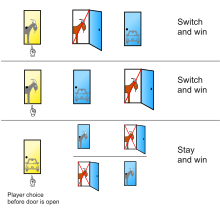
\includegraphics[width=350pt]{imagens/220px-Monty_Hall_Problem_-_Standard_probabilities.svg.png}
    \caption{the paradox of monty hall }~\cite{wikipedia}
    \label{fig:chainimage}
\end{figure}

%%%%%%%%%%%%%%

\chapter{Como os humanos se comportariam dependendo da dificuldade da \ac{IA} em um videogame?}\cite{ia2}
%%%%%%%%%%%%%
Uma vez que se sabe que a \ac{IA} não pode em sua totalidade se comportar igual aos humanos, agora o comportamento dos humanos será visto dependendo da dificuldade da \ac{IA} em diversos videogames.
Os videogames buscam sempre a satisfação do jogador, em sua essência são um instrumento criado para entreter alguém. Para isso, é necessário manter o usuário em um nível equilibrado de desafio e habilidade, pois se o usuário tiver uma habilidade muito inferior ao desafio proposto pelo jogo, o usuário ficará frustrado, enquanto se acontecer exatamente o contrário , o usuário começará a ficar entediado e em algum momento sairá do jogo.\\
    
Este é o verdadeiro problema dos desenvolvedores, que precisam escolher para qual perfil de usuário criarão seu jogo. À medida que mais perfis querem alcançar, mais variantes devem ser geradas pela \ac{IA} dos inimigos, nas habilidades dos personagens, nos elementos do mapa, na forma como eles se comportam dentro daquele espaço e por fim que o jogo não sofra de Quedas de FPS (frames por segundo)
Mas ainda há um problema. O que significa fácil e o que significa difícil? Onde colocamos a régua de medição? Para isso foi criada a dificuldade dinâmica adaptativa. Com isso, o jogo consegue reconhecer as dificuldades que o usuário está sofrendo e aumentar ou diminuir sua dificuldade dependendo de sua habilidade.
Um videogame que usa dificuldade dinâmica adaptativa é Resident Mal 4. Nele, a inteligência dos inimigos é reduzida ao derrotar o jogador diversas vezes consecutivas no mesmo local. Também é usado em Mario Kart 8, aumentando ou reduzindo a probabilidade de diferentes objetos aparecerem nas caixas dependendo da posição atual na corrida (onde na corrida o usuário está por último, é mais provável que ele toque no foguete, mas quando o jogador vai primeiro quase sempre toca a casca da banana)\\
    
A dificuldade dinâmica adaptativa atualmente ainda precisa ser aprimorada. O usuário pode receber ajuda dependendo de seus padrões. Por exemplo, em O Last of Us : Parte 2, se o usuário demorar muito para se deslocar de uma área para outra, será oferecida a possibilidade de receber uma pista. Não há como saber se o usuário realmente precisava dele ou se simplesmente deixou o controle de lado e esperou recebê-lo. Esses tipos de decisões podem afetar a progressão que o jogador obtém à medida que avança no videogame.\\
    
Mas, fora isso, existe o oposto completo, jogos que se baseiam no jogador querer derrubar o controle por raiva por não conseguir passar uma parte do jogo. Existe uma desenvolvedora que leva tudo isso ao limite. Esta empresa é chamada de software
É uma empresa japonesa que desenvolve videogames, teve grande evolução e crescimento na última década com jogos como dark almas , transmitidas pelo sangue , etc. Todos desenvolvidos por seu diretor criativo, Hidetaka Miyazaki, tamanho foi o sucesso e a influência desses jogos na indústria de videogames que nasceu a era dos jogos difíceis ou mais conhecidos como jogos soulslike (terminologia cunhada para definir todos aqueles videogames que são difíceis e tem estilo igual ou semelhante ao escuro alma\\
    
Tem havido muitas pessoas que entram no mundo sombrio de uma era medieval com um tema de fantasia sombria, mas poucos são aqueles que realmente conseguem aproveitar o desafio de passar em um desses jogos.
    
Acima de tudo, pela sua \ac{IA}, que segundo os especialistas é uma das inteligências artificiais mais desenvolvidas em videojogos, pelo nível de desafio que proporciona a quem joga este género de videojogos.
    
Isso pode ser demonstrado com a quantidade infinita de compilações de fúria que existem no YouTube , como as pessoas quase choram por causa do desespero desses jogos que alguns consumidores classificam como diabólicos.

\begin{figure}
    \center
    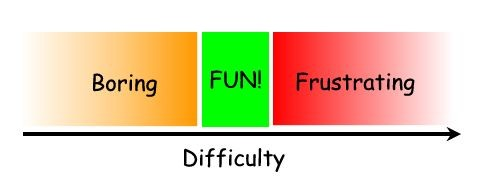
\includegraphics[width=350pt]{imagens/bbd451c375fb5b293a9b1f082bf8d024.jpg}
    \caption{difficulty selector in videogames}~\cite{Vrutal}
    \label{fig:chainimage}
\end{figure}

%%%%%%%
% Conclusões
\chapter{Conclusões}
\label{chap.conclusao}
Em conclusão, exploramos a complexa relação entre \ac{IA} e videogames, questionando se a \ac{IA} pode replicar o comportamento humano. Apesar dos avanços da \ac{IA} nos videogames, ela ainda enfrenta desafios para igualar a complexidade humana. Analisamos como a dificuldade dinâmica adaptativa busca equilibrar o desafio e a satisfação do jogador, enquanto jogos como os Soulslike geram diversas reações, desde satisfação até frustração.

Examinamos a implementação de algoritmos de aprendizado de máquina em videogames, destacando sua capacidade de tomar decisões estratégicas e se adaptar à habilidade do jogador. Também consideramos as futuras etapas da \ac{IA}, desde especializada até geral, e como ela se integra aos videogames. A interação entre humanos e máquinas nos videogames continua sendo um campo intrigante e em constante evolução, com a tecnologia avançando para aprimorar a capacidade da \ac{IA} de se adaptar aos jogadores.

%%%%%%%%
% Contibuições
\chapter*{Contribuições dos autores}
\begin{itemize}

\item O \ac{mp} fez o resumo do relatório, e os capítulos 2 e 3.

\item O \ac{hm} escreveu a introdução e conclusão do trabalho, e o capitulo 4.
\end{itemize}
O \ac{mp} e o \ac{hm} fizeram aproximadamente 50\% do relatório cada um, sendo no final verificado por ambos para confirmar que não existiam erros.

%%%%%%%%%%%%%%%%%%%%%%%%%%%%%%%%%
\chapter*{Acrónimos}
\begin{acronym}
\acro{mp}[MP]{Matheus Pinto}
\acro{hm}[HM]{Henrique Moreira}
\acro{IA}{Inteligência Artificial}
\end{acronym}
%%%%%%%%%%%%%%%%%%%%%%%%%%%%%%%%%
\printbibliography

\end{document}
